% !TEX encoding = UTF-8 Unicode
% !TEX TS-program = pdflatex
% !TEX TS-program = xelatex

\DeclareOldFontCommand{\rm}{\normalfont\rmfamily}{\mathrm}
\DeclareOldFontCommand{\sf}{\normalfont\sffamily}{\mathsf}
\DeclareOldFontCommand{\tt}{\normalfont\ttfamily}{\mathtt}
\DeclareOldFontCommand{\bf}{\normalfont\bfseries}{\mathbf}
\DeclareOldFontCommand{\it}{\normalfont\itshape}{\mathit}
\DeclareOldFontCommand{\sl}{\normalfont\slshape}{\@nomath\sl}
\DeclareOldFontCommand{\sc}{\normalfont\scshape}{\@nomath\sc}
\DeclareRobustCommand*\cal{\@fontswitch\relax\mathcal}
\DeclareRobustCommand*\mit{\@fontswitch\relax\mathnormal}

\documentclass[%
	12pt, 
	a4paper,
	oneside, 
	ngerman,
	bibtotoc,
	dvipsnames,
	table,
]{scrartcl}

\usepackage{wrapfig} 
\usepackage[printonlyused]{acronym}

%\usepackage{tikz}
\usepackage{amssymb,amsmath}
\usepackage{ifxetex,ifluatex}
\usepackage{fixltx2e} % provides \textsubscript
%\usepackage{struktex}

\ifxetex
  \usepackage{fontspec,xltxtra,xunicode}
  \defaultfontfeatures{Mapping=tex-text,Scale=MatchLowercase}
  \newcommand{\euro}{€}
    \usepackage{polyglossia} % -ak-
  \setmainlanguage[%
  	spelling=new,%old
  	latesthyphen=true,%false
	%babelshorthands=true,%false
	]{german} % -ak-
  %\setmainlanguage[variant=american]{english} % -ak-
  \usepackage{xecolor}
\else
  \ifluatex
    \usepackage{fontspec}
    \defaultfontfeatures{Mapping=tex-text,Scale=MatchLowercase}
    \newcommand{\euro}{€}
    \usepackage[ngerman]{babel} % -ak-
    \usepackage{color}
  \else
    \usepackage[utf8]{inputenc}
    \usepackage[TS1,T1]{fontenc} % -ak- T1 für \textdblquotedown
    \usepackage{lmodern} % -ak-
%   \usepackage{tgbonum}	% Bookman
%   \usepackage{tgpagella}	% Palatino
%   \usepackage{tgtermes}	% Times
%   \usepackage{tgschola}	% Century Schoolbook
%   \usepackage{iwona}	% 
%   \usepackage{anttor}
    \usepackage[ngerman]{babel}
    \usepackage{color}    
  \fi
\fi


% Format A4
\typearea[3mm]{13}

% Format A5
%\setlength{\paperwidth}{14.8cm}
%\setlength{\paperheight}{21cm}
%\typearea[2mm]{13}

% Format Taschenbuch
%\setlength{\paperwidth}{12cm}
%\setlength{\paperheight}{19cm}
%\typearea[2mm]{12}

% Format iPad
%\setlength{\paperwidth}{14,5cm}
%\setlength{\paperheight}{19cm}
%\typearea{13}

% Format iPod
%\setlength{\paperwidth}{9cm}
%\setlength{\paperheight}{11,5cm}
%\typearea{14}



\ifxetex
\else
	\usepackage{microtype}
\fi
\raggedbottom
\emergencystretch 0.8em

\definecolor{gcolor}{rgb}{0,0,0} % schwarz

%\usepackage{natbib}
%\bibliographystyle{plainnat}

%\usepackage{biblatex}

%\bibliography{$biblio-files$}

%\usepackage{fancyvrb}

% Redefine labelwidth for lists; otherwise, the enumerate package will cause
% markers to extend beyond the left margin.
\makeatletter\AtBeginDocument{%
  \renewcommand{\@listi}
    {\setlength{\labelwidth}{4em}}
}\makeatother
\usepackage{enumerate}

\usepackage{ctable}
\usepackage{float} % provides the H option for float placement

\usepackage{url}

\usepackage{graphicx}



% We will generate all images so they have a width \maxwidth. This means
% that they will get their normal width if they fit onto the page, but
% are scaled down if they would overflow the margins.
%\makeatletter
%\def\maxwidth{\ifdim\Gin@nat@width>\linewidth\linewidth
%\else\Gin@nat@width\fi}
%\makeatother
%\let\Oldincludegraphics\includegraphics
%\renewcommand{\includegraphics}[1]{\Oldincludegraphics[width=\maxwidth]{#1}}

\usepackage{verbatim}

\usepackage{nameref}


\newcommand{\seclabel}[1]{
\label{sec:#1}
}

\newcommand{\secnameref}[1]{
\nameref{sec:#1}
}

\newcommand{\secnamerefn}[1]{
\ref{sec:#1}: \nameref{sec:#1}
}

\newcommand{\secnamerefnpb}[1]{
Kapitel\secnamerefn{#1}auf Seite \pageref{sec:#1}
}

\newcommand{\secnamerefnpbf}[1]{
Kapitel\secnamerefn{#1}auf Seite \pageref{sec:#1}.
}

\newcommand{\secnamerefnp}[1]{
(Kapitel\secnamerefn{#1}auf Seite \pageref{sec:#1})
}



\usepackage{float}
\floatstyle{boxed}
\restylefloat{figure}

\newcommand{\figref}[1]{
Abb.~\ref{fig:#1}
}

\newcommand{\figreflong}[1]{
Abbildung~\ref{fig:#1}
}

\newcommand{\figrefp}[1]{
\figref{#1} auf Seite~\pageref{fig:#1}
}


% @acuda
% change to alternative figure numbering
% default:  in book class figures are numbered per chapter
%           in article class figures are numbred continuously
%
% change book-class default to continuosly behavior:
% \usepackage{chngcntr}
% \counterwithout{figure}{chapter}
%
% change article-class default to per chapter (section) style:
\usepackage{chngcntr}
%\counterwithin{figure}{section}


% @acuda
% generate new appendix behavior
% now add caption to toc without numbering
\let\Oldappendix\appendix
\def\appendix{
	\Oldappendix
	%\phantomsection 
	\addcontentsline{toc}{section}{Anhang}
	\renewcommand\refname{Anhang} \section*{Anhang}
}

% @acuda #####################
%add for centered captions following options: justification=justified, singlelinecheck=false
\usepackage[font=small, labelfont=bf]{caption}
\usepackage{subcaption}

\KOMAoptions{parskip=half}
%\addtokomafont{caption}{\footnotesize} %lable captions smaller...


\usepackage{blindtext} 

\usepackage{bibgerm}
%\usepackage{titlesec}	%clearpage (newpage with correct floating enviroment) before sections
\newcommand{\sectionbreak}{\clearpage}



\ifxetex
  \usepackage[setpagesize=false, % page size defined by xetex
              unicode=false, % unicode breaks when used with xetex
              xetex,
              bookmarks=true,
              pdfauthor={$author-meta$},
              pdftitle={$title-meta$},
              colorlinks=true,
              urlcolor=blue,
              linkcolor=blue]{hyperref}
\else
  \usepackage[unicode=true,
              bookmarks=true,
              pdfauthor={$author-meta$},
              pdftitle={$title-meta$},
              colorlinks=false,
              urlcolor=blue,
              linkcolor=blue]{hyperref}
\fi
\hypersetup{breaklinks=true, pdfborder={0 0 0}}

\setlength{\emergencystretch}{3em}  % prevent overfull lines


\usepackage{textcomp}

\usepackage{csquotes}

\usepackage{multirow}
\usepackage{pdflscape}

\setcounter{tocdepth}{3}


%%%% Eigene Kopf und Fußzeile %%%%%%%%%%%%%%%% 
%\usepackage{scrpage2}%                              Package laden 
%\pagestyle{scrheadings}%                           SCRPAGE2 Style aktivieren 
%\clearscrheadfoot%                                    lösche alle Kopf und Fußzeilen 
%\setheadwidth{textwithmarginpar}%             für textbreite+rand 
%\automark{chapter}%                                    Autoerkenneung Chapter 
%\ohead{\textbf{\pagemark}}%                      Seitenzahl 
%\renewcommand{\chaptermark}[1]{\markright{\ #1}} %löscht die Nummerierung von Chapter 
%\ihead{\textbf{\rightmark}} 
%%%%%%%%%% Striche Kopfzeile %%%%%%%%%%%%% 
%\setheadtopline{2pt}[\color{blue}] 
%\setheadsepline{1pt}[\color{blue}] 



\usepackage[%
	automark,
	headsepline,                %% Separation line below the header
	%footsepline,               %% Separation line above the footer
	markuppercase
]{scrpage2}
\automark[%
	%subsection  % durch renewcommand gelöst?
]{section}
\pagestyle{scrheadings}
\renewcommand{\sectionmark}[1]{\markright{\ #1}} %löscht die Nummerierung von Chapter 

\lefoot{}                      %% Bottom left on even pages
\lofoot{}                      %% Bottom left on odd pages
\refoot{}                      %% Bottom right on even pages
\rofoot{}                      %% Bottom right on odd pages
\cfoot{--~\pagemark~--}        %% Bottom center
 
%\lehead{\bfseries\pagemark}    %% Top left on even pages
%\lohead{\bfseries\headmark}    %% Top left on odd pages
%\rehead{\bfseries\headmark}    %% Top right on even pages
\rohead{\headmark}    %% Top right on odd pages
\chead{}                       %% Top center
%\renewcommand{\subsectionmark}[1]{\markright{\ #1}} %löscht die Nummerierung von Chapter 


%%%%%%%%%%%%%%%%%%%%%%%%%%%%%%%%%%%%%%%%%%%%%%%%%%%%%
% C M D :   E I G E N N A M E N
%%%%%%%%%%%%%%%%%%%%%%%%%%%%%%%%%%%%%%%%%%%%%%%%%%%%%

\newcommand{\en}[1]{%
\glqq\textit{#1}\grqq%
}


\usepackage{listings}
%\input{listings-python-setup}
%\input{python-function-definition-setup}

\usepackage{setspace}	%zeilenabstand

\makeatletter
\newcommand{\MSonehalfspacing}{%
  \setstretch{1.44}%  default
  \ifcase \@ptsize \relax % 10pt
    \setstretch {1.448}%
  \or % 11pt
    \setstretch {1.399}%
  \or % 12pt
    \setstretch {1.433}%
  \fi
}

\newcommand{\MSdoublespacing}{%
  \setstretch {1.92}%  default
  \ifcase \@ptsize \relax % 10pt
    \setstretch {1.936}%
  \or % 11pt
    \setstretch {1.866}%
  \or % 12pt
    \setstretch {1.902}%
  \fi
}
\makeatother


\onehalfspacing



%%%%%%%%%%%%%%%%%%%%%%%%%
% TEXT ANNOTATIONS		
%%%%%%%%%%%%%%%%%%%%%%%%%

\newcommand{\note}[1]{
\textcolor{orange}{\textbf{Notiz:} #1}
}

\makeatletter
\newcommand{\todo}[1]{
\textcolor{blue}{\textbf{ToDo:} #1}
}




\let\oldcite\cite%
\renewcommand{\cite}[2][]{%
	\ifx&#1&%
		\mbox{\oldcite{#2}}%
	\else%
		\mbox{\oldcite[#1]{#2}}%
	\fi%
}

\newcommand*{\eqcite}[2][]{%
	\vadjust{%
	    \smallskip
	    \hbox to \linewidth{\hfill%
			\ifx&#1&%
				\cite{#2}%
			\else%
				\cite[#1]{#2}%
			\fi%
	    }%
	}%
}%

% Mit diesem Paket können Farben innerhalb von Tabellen verwendet werden. 
% Es können Spalten, Zeile oder einzelne Zellen eingefärbt werden.
\usepackage{colortbl}


\DeclareUnicodeCharacter{20AC}{\euro}


\begin{document}

\thispagestyle{plain}
\begin{titlepage}
\begin{center}
%\begin{figure}[H]
\centering

\includegraphics[scale=2.2]{grafic/logo_hhn_titlepage} \\
\vspace{0.2cm}
\large Fakultät für Mechanik und Elektronik
%\end{figure}
\vspace{0.5cm}
\hrule

\vspace{2cm}

\LARGE{\textbf{\scshape{Digitale Signalverarbeitung und Mustererkennung}}}\\
\vspace{0.3cm}
\LARGE{\textbf{\scshape{(Digitale Signalverarbeitung 2)}}}\\
\vspace{1.8cm}
\Huge{\textbf{Abschlussprojekt\\zur Vorlesung}} \\
%\vspace{1cm}
\vfill


\begin{figure}[H]
	\newlength{\myl}
	\settowidth{\myl}{Lecturer:  }
	\hspace{-\myl}
	\centering
	\large
% \begin{tabular}{|p{3cm}|p{0.09\linewidth}p{0.15\linewidth}p{0.09\linewidth}|}
	\begin{tabular}{llr}
		\textbf{Dozent:} & \multicolumn{2}{l}{Prof. Dr. Volker Stahl} \\
		                   &                &  \\
		\textbf{Autoren:}  & Andreas Schneider   & 198805                     \\
		                   & Gustav Willig    & 197332 \\
		                   & Lisa-Franziska Schäfer	& 199318 \\
	\end{tabular}
\end{figure}

\large

%\vfill
\hrule
%\vspace{0.5cm}
\normalsize
Abgabedatum: Heilbronn, 04. Januar 2017%\today 

\end{center}


\thispagestyle{empty}
	
\end{titlepage}

%\textsf{\textbf{\Large Erklärung der Urheberschaft}}

Hiermit versichern wir, dass die vorliegende Arbeit selbstständig und ohne fremde Hilfe angefertigt wurde. 
Inhalte und Passagen, die aus fremden Quellen stammen, wurden als solche kenntlich gemacht.
Ferner versichern wir, dass keine andere, außer der im Literaturverzeichnis angegebenen Literatur verwendet wurde.
Diese Versicherung bezieht sich sowohl auf Textinhalte sowie alle enthaltenden Abbildungen, Skizzen und Tabellen. 
%Die Arbeit wurde, sowohl in gleicher als auch vergleichbarer Form, bisher keiner Prüfungsbehörde vorgelegt und auch noch nicht veröffentlicht.


\vspace{3em}
\rule{5cm}{0.4pt} \newline
Andreas Schneider

\vspace{1.5em}
\rule{5cm}{0.4pt} \newline
Gustav Willig

\vspace{1.5em}
\rule{5cm}{0.4pt} \newline
Lisa-Franziska Schäfer

\thispagestyle{empty}

%\textsf{\textbf{\Large Statement of authorship}}

%Herewith we assure to have made the present project work without help of third and only with the given sources and aid. All content which was taken from external sources is marked. This work was not presented in same or similar form of an exam authority yet.
%
%\begin{tabbing}
%\hspace{5.9cm}\=\hspace{5.9cm}\=\kill
%\>   \>  \\ 
%\>   \>  \\ 
%\rule{4cm}{0.4pt} \>  \rule{4cm}{0.4pt} \> \rule{4cm}{0.4pt} \\ 
%Mathias Bopp \>  Michael Chrz \> Björn Eistel \\ 
%\>   \>  \\ 
%\>   \>  \\ 
%\>   \>  \\ 
%\rule{4cm}{0.4pt} \>  \rule{4cm}{0.4pt} \>  \\ 
%Felix Herzog \>  Timo Watzka \> 
%\end{tabbing} 

%\vfill
%
%\textsf{\textbf{\Large Abstract}}
%
%if needed....

\typearea[3mm]{13}
\pagenumbering{roman}


%%%%%%%%%%%%%%%%%%%%%%%%%%%%%%%%%%%%%%%%%%%%%%%%%%%%%
% T O C
%%%%%%%%%%%%%%%%%%%%%%%%%%%%%%%%%%%%%%%%%%%%%%%%%%%%%
\begingroup
\tableofcontents
\endgroup

\clearpage
\pagenumbering{arabic}
\setcounter{page}{2} % reset page counter -> titlepage is not counted


\section{Aufgabenstellung}

Im Rahmen der Mastervorlesung \en{Digitale Signalverarbeitung 2} bzw \en{Digitale Signalverarbeitung und Mustererkennung} soll ein Abschlussprojekt bearbeitet werden, um die aus der Vorlesung gewonnenen theoretischen Erkenntnisse praktisch anzuwenden. 
Ziel des Projekts ist es ein Programm zur einfachen Spracherkennung zu realisieren. 
Zudem sollen am Computer einige Experimente durchgeführt und in dem vorliegenden Abschlussprojektbericht dokumentiert werden. 


\newpage 

\section{Planung und Vorbereitungen}

Die Bearbeitung der Projektaufgabe erfolgt in der Programmsprache \en{Python}, da die Gruppenmitglieder hier bereits einige Vorkenntnisse mitbringen. 
Ein weiterer Vorteil von Python ist dessen Plattformunabhängigkeit, wodurch das Projekt ohne Anpassungen sowohl auf Linux- als auch auf Windows-Betriebssystemen lauffähig ist.

Zum Trainieren von verschiedenen Modellen wurden zunächst die Wörter in der nachfolgenden Tabelle \ref{tab:recorded_words} erzeugt.
Für jedes Wort liegen insgesamt 54 Merkmalsvektorfolgen vor.
Dabei stammen jeweils 36 von zwei männlichen Sprechern und 18 von einer weiblichen Sprecherin. 
Um die Abhängigkeit der Klassifikationsqualität von der Umgebung zu vermindern, wurden die Aufnahmen zur Hälfte in einer ruhigen Umgebung (G117) und mit Hintergrundgeräuschen (A409, laufender Beamer) gesprochen. 
Weiterhin wurde eine Aufnahme der im jeweiligen Raum herrschenden \en{Stille} erzeugt.


\bigskip
{\setlength{\extrarowheight}{2pt}%
\begin{table}[!hp]
\centering
\begin{tabular}{| c | l |}
\hline
Namen		 & Andreas, Gustav, Lisa  \\ \hline
Zahlen		 & Zwei, Drei               \\ \hline
Hausaufgaben & Signalverarbeitung, Fouriertransformation \\ \hline
sonstige 	 & mögen, und 	\\ \hline
\end{tabular}
\caption[Erzeugte Merkmalsvektorfolgen]{Erzeugte Merkmalsvektorfolgen}
\label{tab:recorded_words}
\end{table}
\bigskip



\begin{comment}
Die Berechnung der Distanzen kann durch verschiedene Methoden erfolgen. Folgenden Methoden wurden verwendet:

\begin{itemize}
	\item Euklidischer Abstand
	\item Mahalanobis Abstand
	\item Abstandsmaß basierend auf der Normalverteilung
	\item HMM (als Produktfolge)
	\item HMM (Maximum Approximation)
	\item HMM (negativ logarithmierte Wahrscheinlichkeiten)
\end{itemize}
\end{comment}
\newpage

\section{Klassifikation}

Da die Software im Laufe des Projektes stetig weiterentwickelt wurde, steht zur Berechnung der Kosten bzw. Wahrscheinlichkeiten nur die am Besten funktionierende Methode zur Verfügung, \en{HMM mit maximum Approximation}.

\note{Bei Einzelwörtern hat der Sprecher ein besseres Ergebnis als All. Bei Wortfolgen schneidet das Modell All besser ab, als der eigentliche Sprecher!}

\subsection{Einzelworterkennung}

Die folgenden Tabellen zeigen ...


\begin{table}[!hp]
\centering
%\rowcolors{1}{RoyalBlue!20}{RoyalBlue!5}
\begin{tabular}{|l|l|l|l|}
\hline
Stillemodell 			& Referenzmodell 	  & Getestetes Wort 	& Kosten \\ \hline \hline
\rowcolor{green!50} A409& Drei\_Andreas\_A409 & Drei\_Andreas 	& -168,04 \\ \cline{3-4}
						&				 	  & Drei\_Gustav  	&  198,98 \\ \cline{3-4}
						&					  & Drei\_Lisa	  	&  113,26 \\ \hline \hline
A409					& Drei\_All\_409	  & Drei\_Andreas 	& -95,74 \\ \cline{3-4}
						&				 	  & Drei\_Gustav  	& -46,10 \\ \cline{3-4}
\rowcolor{green!50}		&					  & Drei\_Lisa	  	& -112,95 \\ \hline \hline
\rowcolor{green!50} G117& Drei\_Andreas\_A409 & Drei\_Andreas 	& -179,47 \\ \cline{3-4}
						&				 	  & Drei\_Gustav  	& 89,10\\ \cline{3-4}
						&					  & Drei\_Lisa	  	& 12,85 \\ \hline \hline
G117					& Drei\_All\_A409	  & Drei\_Andreas 	& -105,82 \\ \cline{3-4}
						&				 	  & Drei\_Gustav  	& -57,20 \\ \cline{3-4}
\rowcolor{green!50}		&					  & Drei\_Lisa	  	& -125,85  \\ \hline \hline
\end{tabular}
\caption[Getestete Prädiktion für das Stillemodell A409]{Getestete Prädiktion für das Stillemodell A409}
\label{tab:predict_G117}
\end{table}


\begin{table}[!hp]
\centering
\rowcolors{1}{RoyalBlue!20}{RoyalBlue!5}
\begin{tabular}{|l|l|l|l|l|}
\hline
Stillemodell & Getestet	für 	 			 & Wort 	 & Sprecher & Kosten \\\hline\hline
A409        & Signalverarbeitung\_Gustav\_G117 & Signalverarbeitung & Gustav &  230,60		\\ \hline
G117		& Signalverarbeitung\_Gustav\_G117 & Signalverarbeitung	& Gustav & 225,27	\\ \hline
A409		& Zwei\_Lisa\_A409				 & Zwei & Lisa & -210,28	\\ \hline
G117		& Zwei\_Lisa\_A409				 & Zwei & Lisa & -235,00 \\ \hline
\end{tabular}
\caption[Prädiktion mit Sprechererkennung]{Prädiktion mit Sprechererkennung}
\label{tab:predict_all_modells}
\end{table}

\newpage
\begin{table}[!hp]
\centering
\rowcolors{1}{RoyalBlue!20}{RoyalBlue!5}
\begin{tabular}{|l|l|l|l|}
\hline
Stillemodell & Getestet	für 	 			 & Wort 	 & Kosten \\\hline\hline
A409        & Signalverarbeitung\_Gustav\_G117 & Signalverarbeitung  & 447,73  		\\ \hline
G117		& Signalverarbeitung\_Gustav\_G117 & Signalverarbeitung & 442,40	\\ \hline
A409		& Zwei\_Lisa\_A409			& Zwei & 28,13	\\ \hline
G117		& Zwei\_Lisa\_A409			& Zwei & 21,17	\\ \hline
\end{tabular}
\caption[Prädiktion mit veralgemeinerten Modellen]{Prädiktion mit veralgemeinerten Modellen}
\label{tab:predict_ALL}
\end{table}



\bigskip
\subsection{Wortfolgenerkennung}

Da es wie bei der Einzelworterkennung kaum einen Unterschied zwischen dem verwendetem Stillemodell gibt, werden für die folgenden Tests nur G117 verwendet.
Aufgrund der sonst übergroßen Breite der Tabellen wird das Wort \en{Fouriertransformation} mit FT und \en{Signalverarbeitung} mit SV abgekürzt.

\begin{table}[!hp]
\centering
\rowcolors{1}{RoyalBlue!20}{RoyalBlue!5}
\begin{tabular}{|l||l|l|l|}
\hline
Gesprochenes Wort & Andreas & Gustav  & Lisa 	\\\hline\hline
Lisa     		   & Lisa 	 & Lisa	   & Lisa	\\ \hline
und		  		   & und  	 & und	   & und	\\ \hline
Gustav			   & Gustav  & Gustav  & Gustav	\\ \hline
und				   & 	 	 & und	   & und	\\ \hline
Andreas			   & Andreas & Andreas & Andreas\\ \hline
mögen			   & mögen	 & mögen   & mögen	\\ \hline
SV				   & SV		 & SV	   & SV	\\ \hline
\end{tabular}
\caption[Prädiktion mit veralgemeinerten Modellen]{Prädiktion mit veralgemeinerten Modellen}
\label{tab:predict_ALL_1}
\end{table}

\begin{table}[!hp]
\centering
\rowcolors{1}{RoyalBlue!20}{RoyalBlue!5}
\begin{tabular}{|l||l|l|l|l|l|l|}
\hline
Gesprochenes Wort & \multicolumn{2}{|c|}{Andreas} & \multicolumn{2}{|c|}{Gustav} & \multicolumn{2}{|c|}{Lisa} \\ \hline
		& Wort	 & Sprecher& Wort	& Sprecher & Wort 	& Sprecher\\	\hline \hline
Lisa    & Lisa 	 & Andreas & Lisa	& Gustav   & Lisa	& Lisa	\\ \hline
und		& und  	 & Andreas & und	& Gustav   & und	& Lisa	\\ \hline
Gustav	& Gustav & Andreas & Gustav & Gustav   & Gustav	& Lisa	\\ \hline
und		& 	 	 & 		   & und	& Gustav   & und	& Lisa	\\ \hline
Andreas	& Andreas& Andreas & Andreas& Andreas  & Andreas& Andreas \\ \hline
mögen	& mögen	 & Gustav  & mögen  & Gustav   & mögen	& Lisa	\\ \hline
SV		& SV	 & Andreas & SV	    & Gustav   & SV		& Lisa	\\ \hline
\end{tabular}
\caption[Prädiktion mit Sprechererkennung]{Prädiktion mit Sprechererkennung}
\label{tab:predict_Speaker_1}
\end{table}

\newpage

\begin{table}[!hp]
\centering
\rowcolors{1}{RoyalBlue!20}{RoyalBlue!5}
\begin{tabular}{|l||l|l|l|}
\hline
Gesprochenes Wort & Andreas & Gustav & Lisa 		\\\hline\hline
				   & 		 & moegen & drei	\\ \hline
und       		   & und 	 & und	  & und		\\ \hline
und				   & und  	 & und	  & und			\\ \hline
				   & 		 & drei	  & \\ \hline
FT 				   & FT 	 & FT 	  & FT\\ \hline
zwei			   & zwei 	 & zwei   & zwei	\\ \hline
drei			   & drei	 & drei   & drei	\\ \hline
\end{tabular}
\caption[Prädiktion mit veralgemeinerten Modellen]{Prädiktion mit veralgemeinerten Modellen}
\label{tab:predict_ALL_2}
\end{table}

\begin{table}[!hp]
\centering
\rowcolors{1}{RoyalBlue!20}{RoyalBlue!5}
\begin{tabular}{|l||l|l|l|l|l|l|}
\hline
Gesprochenes Wort & \multicolumn{2}{|c|}{Andreas} & \multicolumn{2}{|c|}{Gustav} & \multicolumn{2}{|c|}{Lisa} \\\hline
	& Wort & Sprecher & Wort & Sprecher & Wort   & Sprecher \\ \hline \hline
	& und  & Andreas  & drei & Andreas  & zwei   & Andreas	\\ \hline
und & und  & Gustav	  & und	 & Gustav   & und    & Lisa	\\ \hline
und	& und  & Andreas  & und	 & Gustav   & und    & Lisa	\\ \hline
	& 	   & 		  & drei & Andreas  & 	     & 	\\ \hline
FT 	&  FT  & Andreas  & FT 	 & Gustav   & Andreas& Andreas \\ \hline
zwei& drei & Andreas  & drei & Andreas  & zwei   & Lisa \\ \hline
drei& drei & Andreas  & drei & Gustav   & drei   & Lisa \\ \hline
\end{tabular}
\caption[Prädiktion mit Sprechererkennung]{Prädiktion mit Sprechererkennung}
\label{tab:predict_ALL_2}
\end{table}



\note{je größer die Pause zwischen den einzelnen Worten desto besser das Klassifikationsergebnis}
\newpage

%\section{Experimente}

%Unterscheidung zwischen männlein und weiblein

%Laufzeit Training, Prädiktion


\newpage
\section{GUI}

Zur besseren Bedienbarkeit des Programms wurde eine graphische Benutzeroberfläche entwickelt.
Diese ermöglicht es mit geringem Aufwand, Modelle aus den vorhandenen Merkmalsvektorfolgen zu trainieren sowie zu testen.
%Konfigurationen zu tätigen und die gewünschten Funktionen zu starten.
Hierdurch wird der Umgang mit den Datenmengen sowie die Durchführung von Experimenten vereinfacht. % das Erzeugen von Grafiken und Auswertungen. 
Die Benutzeroberfläche ist in der Abbildung \ref{fig:gui} dargestellt.


\medskip
\begin{figure}[tbph!]
\centering
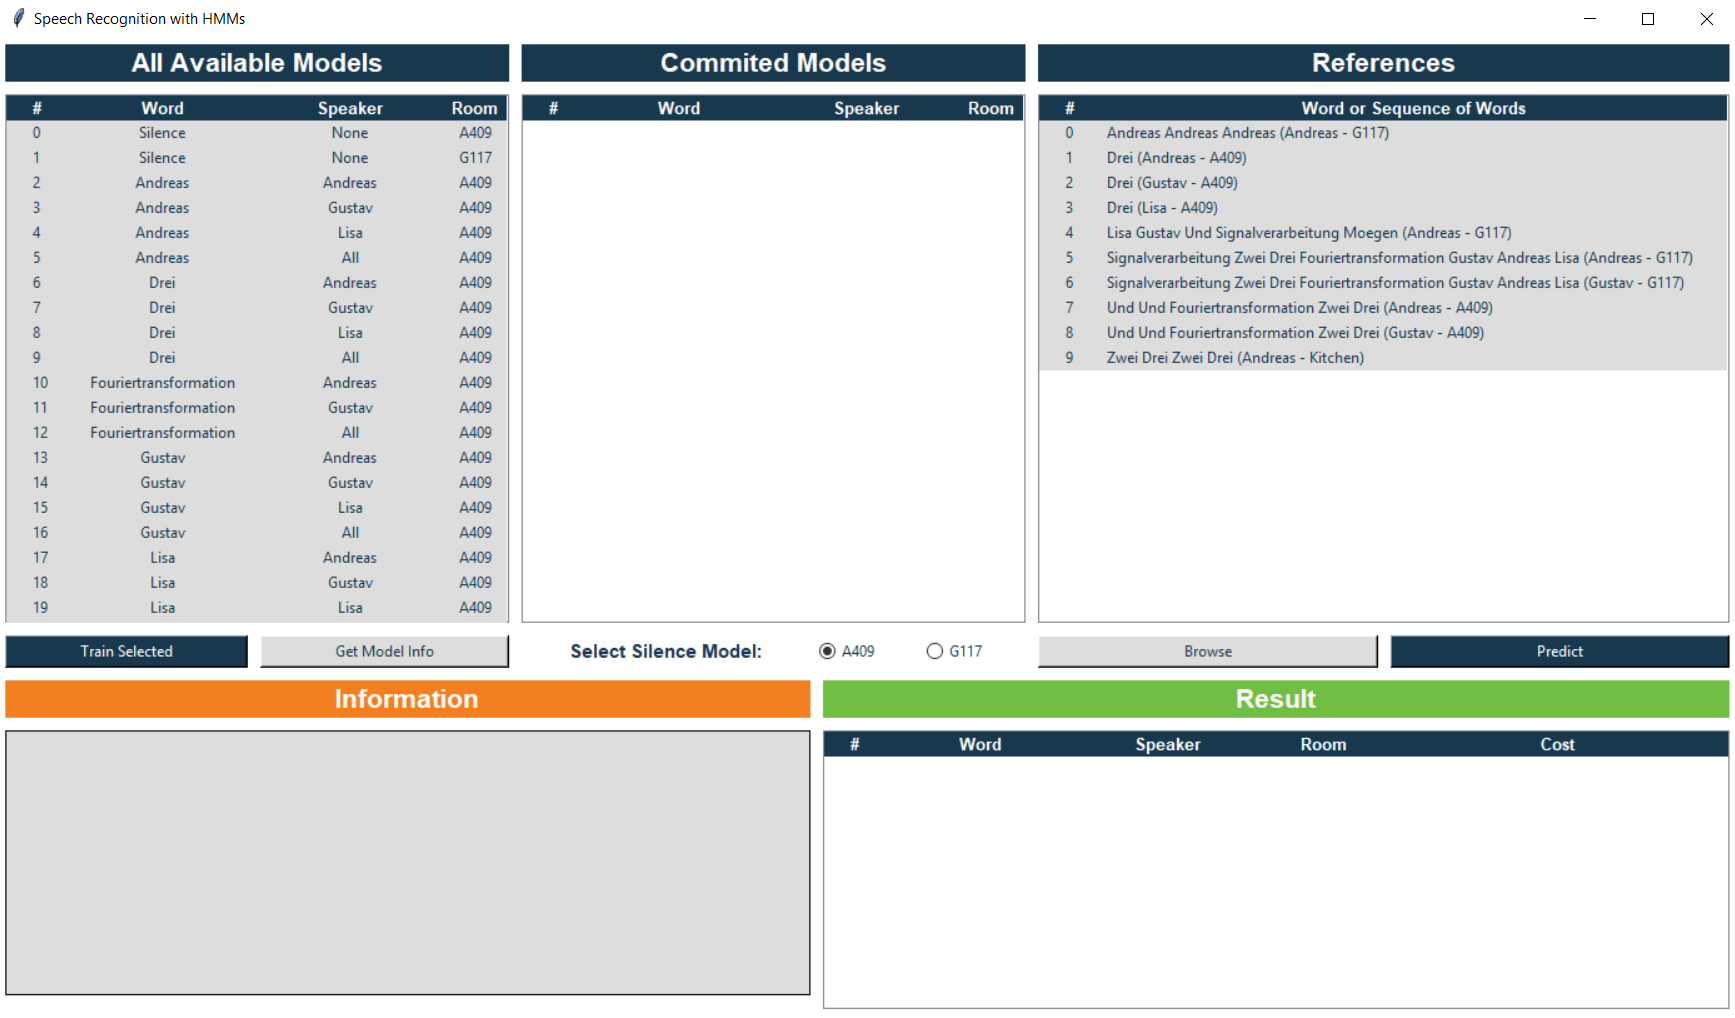
\includegraphics[width=0.92\linewidth]{grafic/gui}
\caption{grafische Benutzeroberfläche}
\label{fig:gui}
\end{figure}


In der linken oberen Box sind alle verfügbaren Modelle aufgelistet.
Über die beiden darunter liegenden Buttons können die Modelle entweder neu trainiert oder Informationen, wie z.B. die Modelllänge oder die benötigten Iterationen, angezeigt werden.
Die mittlere Box zeigt die aktuell für die Klassifikation zur Auswahl stehenden Modelle an.
Durch einen Doppelklick auf ein Modell in der linken Box, kann dieses für die später folgende Prädiktion geladen werden.
Das zu verwendende Stillemodell wird über die darunter angeordneten Radiobuttons ausgewählt.

Um ein Wort durch die Software klassifizieren zu lassen, muss dieses durch den Button \en{Browse} in die obere rechte Box geladen und ausgewählt werden.
Hierdurch können auch gesprochene Wortfolgen ausgewertet werden.
Zum Starten der Prädiktion wird der Button \en{Predict} betätigt, das Ergebnis wird danach rechts unten angezeigt.
Hierbei wird sowohl das erkannte Wort, als auch der ermittelte Sprecher und die benötigten Kosten aufgelistet. 





% wortfolgen laden und testen
% informationen zu modellen 
% stille modell 
% kosten anschauen




\newpage


%\clearpage
%\listoffigures

%\clearpage
%\listoftables


%%%%%%%%%%%%%%%%%%%%%%%%%%%%%%%%%%%%%%%%%%%%%%%%%%%%%
% L I S T   O F   A C R O N Y M S
%%%%%%%%%%%%%%%%%%%%%%%%%%%%%%%%%%%%%%%%%%%%%%%%%%%%%

% @acuda
% Append Acronym-List in Document with \appendix
% for old behavior use \Oldappendix
% acronym should be the name of the appendix file (linux sort hack)
% linux hack: sort unsort.tex -o sorted.tex (should called via sh-script)
% appendix-file entry: \acro{VERWEIS}[ABKÜRZUNG]{AUSGESCHRIEBEN}
% use acronym:
%   \ac{lable}      full name only at first usage in text
%   \acs{lable}     short name only
%   \acf{lable}     short and full name only
%   \acl{lable}     full name only
%\clearpage
%\phantomsection \addcontentsline{toc}{section}{Acronyms}
%\begingroup
%	\renewcommand\refname{Acronyms} \section*{Acronyms}
%	\sectionmark{Acronyms}
%	% Format der Abkürzungsdefinition: \acro{}[]{}
%	% {Verweis}[Abkürzung]{ausgeschriebene Abkürzung}
%	\begin{acronym}[Library-BindingW] %NMWC YTM
%		\leftskip1.5em
%		\setlength{\itemsep}{-\parsep}
%			\acro{dm}[DM]{dm-drogerie markt GmbH + Co. KG}
%			\acro{eu}[EU]{European Union}
%			\acro{gbs}[GBS]{\en{Green Bag Solutions GmbH}}
%			\acro{kik}[KiK]{KiK Textilien und Non-Food GmbH}
%			\acro{smart}[SMART]{Specific Measurable Accepted Realistic and Time}
%			\acro{wbs}[WBS]{\en{Work Breakdown Structure}}
%			\acrodefplural{wbs}[WBSs]{\en{Work Breakdown Structures}}
%			\acro{lip}[LiP]{\en{Leading in Projects}}
%	\end{acronym}
%\endgroup


%\clearpage
%{
%\renewcommand{\refname}{Bibliography}
%\bibliographystyle{alphadin}
%\bibliography{source/source} 
%}
%
%
%\clearpage
%\input{appendix/_appendix}


\end{document}
